% 92-18(92쪽) — 높이 5 cm 인 원기둥 모양의 컵과 밑면의 원 위의 세 점 A, B, C(원문 「오른쪽 그림」). 스캔 화질이 낮고 색 입체 그림이라 TikZ 로 다시 그림.
% 라벨은 원문 것만: 꼭짓점 A·B·C, 3 cm, 5 cm, 85°, 65°. 컵의 부피(답)가 읽히지 않게 반지름·눈금은 적지 않는다.
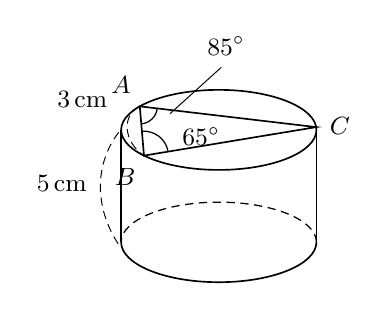
\begin{tikzpicture}[line width=0.6pt, x=0.62cm, y=0.62cm]
  \coordinate (A) at (-1.618,0.482);
  \coordinate (B) at (-1.532,-0.527);
  \coordinate (C) at (1.995,0.057);
  % 컵: 윗면 원 · 옆면 · 밑면(앞은 실선, 뒤는 점선)
  \draw (0,0) ellipse [x radius=2, y radius=0.82];
  \draw (-2,0) -- (-2,-2.3);
  \draw (2,0) -- (2,-2.3);
  \draw (-2,-2.3) arc [start angle=180, end angle=360, x radius=2, y radius=0.82];
  \draw[densely dashed, line width=0.45pt] (2,-2.3) arc [start angle=0, end angle=180, x radius=2, y radius=0.82];
  % 삼각형 ABC
  \draw (A) -- (B) -- (C) -- cycle;
  % 각 표시
  \draw[line width=0.45pt] ([shift={(-85.1:0.36)}]A) arc [start angle=-85.1, end angle=-6.7, radius=0.36];
  \draw[line width=0.45pt] ([shift={(9.4:0.50)}]B) arc [start angle=9.4, end angle=94.9, radius=0.50];
  \draw[line width=0.35pt] (0.05,1.28) -- (-1.00,0.33);
  % 길이 표시의 점선 호
  \draw[densely dashed, line width=0.35pt] (A) .. controls (-2.00,0.30) and (-1.95,-0.25) .. (B);
  \draw[densely dashed, line width=0.35pt] (-2.05,-0.05) .. controls (-2.55,-0.70) and (-2.55,-1.60) .. (-2.05,-2.35);
  \node[font=\small, anchor=south east] at (-1.60,0.53) {$\pt{A}$};
  \node[font=\small, anchor=north east] at (-1.50,-0.58) {$\pt{B}$};
  \node[font=\small, anchor=west] at (2.07,0.07) {$\pt{C}$};
  \node[font=\small, anchor=south] at (0.15,1.32) {$85^\circ$};
  \node[font=\small, anchor=west] at (-0.95,-0.14) {$65^\circ$};
  \node[font=\small, anchor=east] at (-2.08,0.62) {$3\,\mathrm{cm}$};
  \node[font=\small, anchor=east] at (-2.50,-1.10) {$5\,\mathrm{cm}$};
\end{tikzpicture}
